%%%%%PLEASE CONSIDER CORRECTIONS AT PLACES INDICATED%%%%%%%%
\documentclass{article}
%%%%%Packages Used, add more if necessary%%%%
\usepackage{amsmath,amsfonts,amssymb,graphicx,fullpage}
\setlength{\topmargin}{-0.6 in}
\setlength{\textheight}{8.5 in}
\setlength{\headsep}{0.75 in}
\usepackage{mdframed}
\usepackage{multicol}
\usepackage{microtype}
\usepackage{float}
\usepackage{subcaption}
\usepackage{hyperref}
\usepackage{cite}
\newcommand{\vecb}[1]{\boldsymbol{#1}} % bold Greek / symbols
\newcommand{\matb}[1]{\mathbf{#1}}     % bold matrices
\newcommand{\vb}[1]{\mathbf{#1}}       % bold vectors (latin)

%%%%% NO NEED TO EDIT THIS PREAMBLE %%%%%%%%
%%% PREAMBLE %%%
\newcounter{lecnum}
\renewcommand{\thepage}{\thelecnum-\arabic{page}}
\renewcommand{\thesection}{\thelecnum.\arabic{section}}
\renewcommand{\theequation}{\thelecnum.\arabic{equation}}
\renewcommand{\thefigure}{\thelecnum.\arabic{figure}}
\renewcommand{\thetable}{\thelecnum.\arabic{table}}
\newcommand{\lecture}[4]{
   \pagestyle{myheadings}
   \thispagestyle{plain}
   \newpage
   \setcounter{lecnum}{#1}
   \setcounter{page}{1}
   \noindent
   \begin{center}
   \framebox{
      \vbox{\vspace{2mm}
      
      \hbox to 6.28in { 
      {\bf ECE 4252/6252 (FunML) Fundamentals of Machine Learning \hfill 2021--2028} }
      
      \vspace{2mm}
      \hbox to 6.28in { 
      {Courses developed by Professor Ghassan AlRegib 
      (\href{https://alregib.ece.gatech.edu/}{alregib.ece.gatech.edu}) 
      \hfill For inquiries: \href{mailto:alregib@gatech.edu}{alregib@gatech.edu}} }
      
      \vspace{3mm}
      \hbox to 6.28in { {\Large \hfill Lecture #1: #2 \hfill} }
      
      \vspace{2mm}
      \hbox to 6.28in { {\it Co-Instructors: #3 \hfill #4} }
      
      \vspace{2mm}}
   }
   \end{center}

   % -------- PEOPLE OUTSIDE BOX --------
   \vspace{2mm}
   \noindent{\bf Contributors:} Dr. Ahmad Mustafa, Dr. Motaz Alfarraj, Dr. Ashraf Alattar, Dr. Chen Zhou

   \vspace{1mm}
   \noindent{\bf Teaching Assistants} with remarkable contributions include: Kuo-Wei Lai, Wuyang Du, Shiva Mahato, Michael Zhou, Ninghan Zhong

   \markboth{Lecture #1: #2}{Lecture #1: #2}

   \vspace{2mm}
\noindent {\bf Disclaimer}: 
{All content of these notes are part of this course at Georgia Tech. Any re-use or distribution is not permitted without pre-approved permission. All these notes belong to, created by, and copyrighted for Ghassan AlRegib and Mohit Prabhushankar, Georgia Tech, 2021--2028.}



\vspace{2mm}
\noindent {\bf License}: 
{These lecture notes are licensed under the 
\href{https://creativecommons.org/licenses/by-nc-sa/4.0/}{Creative Commons Attribution-NonCommercial-ShareAlike 4.0 International License}.}

   \vspace{2mm}
   \noindent {\bf Errata}: 
   {\it Please submit any errata you find using the following form: 
   \href{https://forms.office.com/r/fbg9dMWPgY}{Errata Form for FunML Textbook} 
   or visit: \url{https://forms.office.com/r/fbg9dMWPgY}}

   \vspace*{4mm}
}
% \renewcommand{\cite}[1]{[#1]}
% \def\beginrefs{\begin{list}
%         {[\arabic{equation}]}{\usecounter{equation}
%          \setlength{\leftmargin}{2.0truecm}\setlength{\labelsep}{0.4truecm}%
%          \setlength{\labelwidth}{1.6truecm}}}
% \def\endrefs{\end{list}}
% \def\bibentry#1{\item[\hbox{[#1]}]}

\newcommand{\challenge}[2]{\noindent \textbf{(Challenge Problem)} \emph{#1}: #2 }

\newcommand{\exercise}[1]{\noindent \textbf{(Exercise)} #1 }

\newcommand{\fig}[3]{
			\vspace{#2}
			\begin{center}
			Figure \thelecnum.#1:~#3
			\end{center}
	}
%%% END_OF_PREAMBLE %%%


	
%%%%You may add more \newtheorem if necessary%%%%%%
\newtheorem{theorem}{Theorem}[lecnum]
\newtheorem{lemma}[theorem]{Lemma}
\newtheorem{proposition}[theorem]{Proposition}
\newtheorem{claim}[theorem]{Claim}
\newtheorem{corollary}[theorem]{Corollary}
\newtheorem{definition}[theorem]{Definition}
\newenvironment{proof}{{\bf Proof:}}{\hfill\rule{2mm}{2mm}}


\newcommand{\dom}{\mathrm{dom}}

\begin{document}
\lecture{9 (Extension)}{Performance Metrics for Regression}{Ghassan AlRegib and Mohit Prabhushankar}{}

\noindent

This extension to Lecture 9 focuses on evaluating regression models using performance metrics and validation techniques. While Lecture 9 covers optimization and regularization techniques, this document introduces the most commonly used performance metrics for regression. These metrics quantify how well a trained model fits the data and generalizes to unseen examples.

After training a regression model, we need quantitative ways to evaluate how well it performs. The following metrics are commonly used to assess how well model predictions match the true target values. Different metrics capture distinct aspects of prediction quality, such as error magnitude, robustness to outliers, or explained variance. As a result, multiple metrics are often reported together in practice.

\section{Lecture Objectives}

By the end of this extension, you should be able to:

\begin{itemize}
    \item Define and interpret common regression performance metrics (MSE, RMSE, MAE, $R^2$)
    \item Compare metrics based on sensitivity to outliers and interpretability
    \item Apply model validation techniques including train/validation/test splits and cross-validation
    \item Diagnose underfitting and overfitting using learning curves
    \item Understand the relationship between model complexity and generalization error
\end{itemize}

\section{Performance Metrics}

\subsection{Mean Squared Error (MSE)}

The \textbf{Mean Squared Error (MSE)} is one of the most common metrics for regression.  
It measures the average squared difference between predicted values and true values.

\[
\text{MSE}(\matb{X},\vecb{\theta})=\frac{1}{N}\sum_{i=1}^{N}(\hat{y}_i-y_i)^2
\]

where $\hat{y}_i=\vecb{\theta}^T\vb{x}_i$ is the predicted value.

Squaring the error has two important effects:

\begin{itemize}
\item Large errors are penalized more heavily than small errors.
\item The function is smooth and differentiable, making it convenient for optimization.
\end{itemize}

However, because errors are squared, MSE can be sensitive to outliers.

\subsection{Root Mean Squared Error (RMSE)}

The \textbf{Root Mean Squared Error (RMSE)} is the square root of the MSE:

\[
\text{RMSE}(\matb{X},\vecb{\theta})=\sqrt{\frac{1}{N}\sum_{i=1}^{N}(\hat{y}_i-y_i)^2}
\]

RMSE has the same units as the target variable, making it easier to interpret than MSE.  
For example, if the target variable is measured in dollars, RMSE is also measured in dollars.

\subsection{Mean Absolute Error (MAE)}

The \textbf{Mean Absolute Error (MAE)} measures the average magnitude of prediction errors:

\[
\text{MAE}(\matb{X},\vecb{\theta})=\frac{1}{N}\sum_{i=1}^{N}|\hat{y}_i-y_i|
\]

Unlike MSE, MAE does not square the error. This makes MAE:

\begin{itemize}
\item More robust to outliers
\item Less sensitive to large individual errors
\end{itemize}

In practice, MAE and MSE are often reported together to better understand model behavior.

\subsection{Coefficient of Determination ($R^2$)}

The \textbf{Coefficient of Determination} ($R^2$) measures how well the model explains the variance in the target variable.  
It compares the prediction error of the model to the error of a baseline model that always predicts the mean of the target variable.

\[
R^2 = 1 - \frac{SS_{\text{res}}}{SS_{\text{tot}}}
\]

where

\[
SS_{\text{res}}=\sum_{i=1}^{N}(y_i-\hat{y}_i)^2
\]
\[
SS_{\text{tot}}=\sum_{i=1}^{N}(y_i-\bar{y})^2
\]

Interpretation:

\begin{itemize}
\item \textbf{$R^2 = 1$}: Perfect predictions.
\item \textbf{$R^2 = 0$}: Model performs no better than predicting the mean.
\item \textbf{$R^2 < 0$}: Model performs worse than the mean predictor.
\end{itemize}

$R^2$ provides a normalized measure of performance and is especially useful when comparing different models on the same dataset.


\subsection{Summary of Metrics}

To better understand how these metrics relate to each other, we summarize their key properties below. Each metric captures different properties of model performance:
\begin{itemize}
\item MSE and RMSE penalize large errors more heavily.
\item MAE is more robust to outliers and less sensitive to large deviations.
\item $R^2$ measures how much variance in the target variable is explained by the model.
\end{itemize}


\section{Model Validation}

Machine learning models must be evaluated carefully to ensure they generalize to unseen data. In this section, we focus on the procedures used for model validation and generalization assessment. Throughout this section, we refer to evaluation in terms of error for consistency. In general, other metrics (e.g., accuracy or $R^2$) may also be used depending on the task.

% Machine learning models must be evaluated carefully to ensure they generalize to unseen data. 
% This section introduces the core tools used to assess model performance and diagnose common 
% issues such as underfitting and overfitting. We discuss dataset splitting, learning curves, 
% cross-validation, model complexity, and the bias–variance tradeoff.

\subsection{Training/Validation/Test Split}

The test set is kept completely separate from model training and validation. Its purpose is to evaluate performance on unseen data and simulate real-world deployment. By assessing the model on this independent dataset, we ensure that the evaluation reflects real-world generalization performance.


It is critical that the \textbf{test set is never used during model development}. 
If the test set influences model design or hyperparameter tuning, the evaluation 
becomes biased and overly optimistic. The test set should only be used once, 
after the final model has been selected.

The training dataset is where the model learns. It’s typically divided into two parts:

\begin{enumerate}
    \item Training Data: The larger portion used to teach the model by adjusting its parameters based on the loss function.
    \item Validation Data: A smaller portion used to monitor the model's performance during training. It helps fine-tune hyperparameters and assess the risk of overfitting by providing an unbiased evaluation.
\end{enumerate}

The validation subset serves as a checkpoint during training. It helps identify issues like overfitting and informs adjustments to model design and hyperparameters. This ensures that the model remains robust and can generalize well to new data. Typically, 20–30\% of the dataset is reserved for testing, while the remaining 
data is used for training and validation.
\begin{figure}[H]
    \centering
    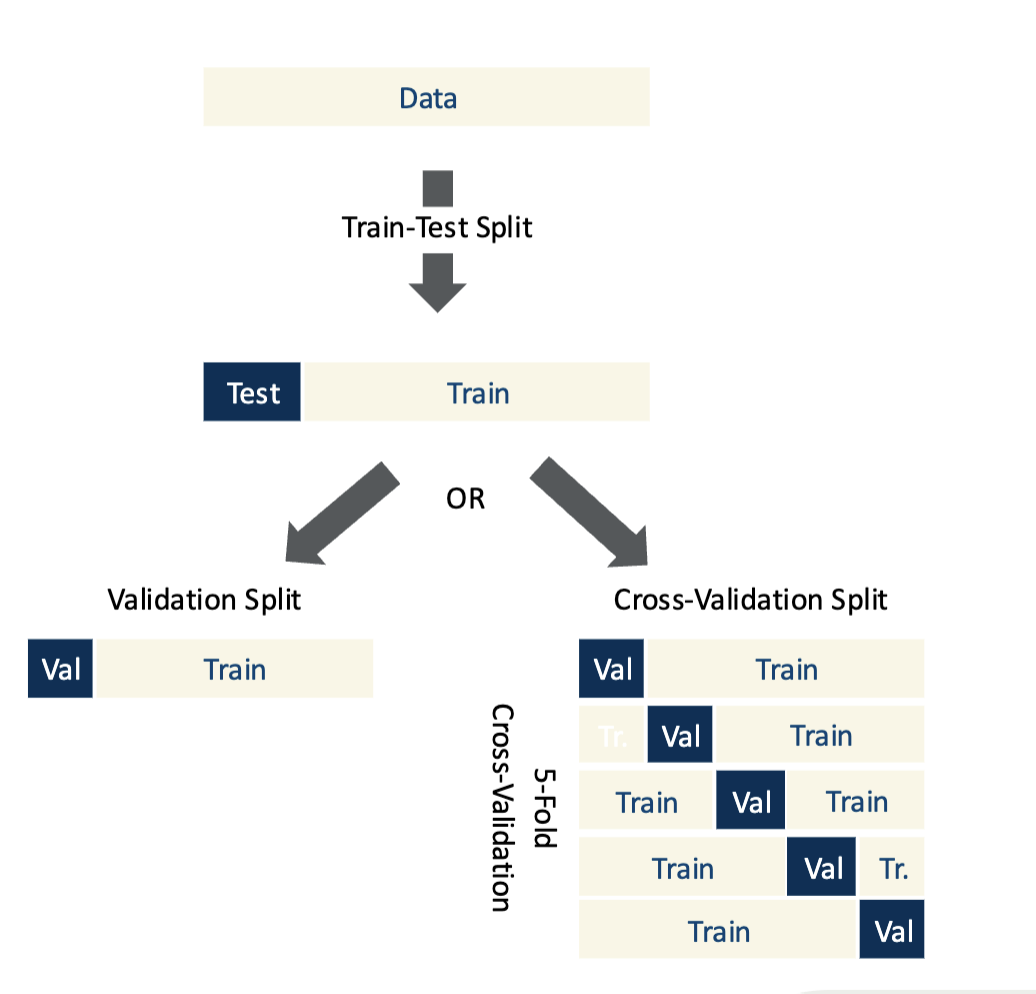
\includegraphics[width=0.5\linewidth]{img/lecture9/Screenshot 2024-09-22 at 6.02.54 PM.png}
    \caption{Visualization of dataset split}
\end{figure}


\paragraph{K-fold Cross-Validation Procedure}

A widely used approach for hyperparameter tuning is $k$-fold cross-validation.
The procedure is:

\begin{enumerate}
    \item Shuffle the dataset randomly.
    \item Split the dataset into $k$ roughly equal subsets (folds).
    \item For each fold:
    \begin{itemize}
        \item Use the fold as the validation set.
        \item Use the remaining $k-1$ folds as the training set.
        \item Train the model and record the validation error.
    \end{itemize}
    \item Average the validation errors across all folds.
\end{enumerate}

After cross-validation, the model is retrained on the full training data
before final evaluation on the test set.

\begin{figure}[H]
    \centering
    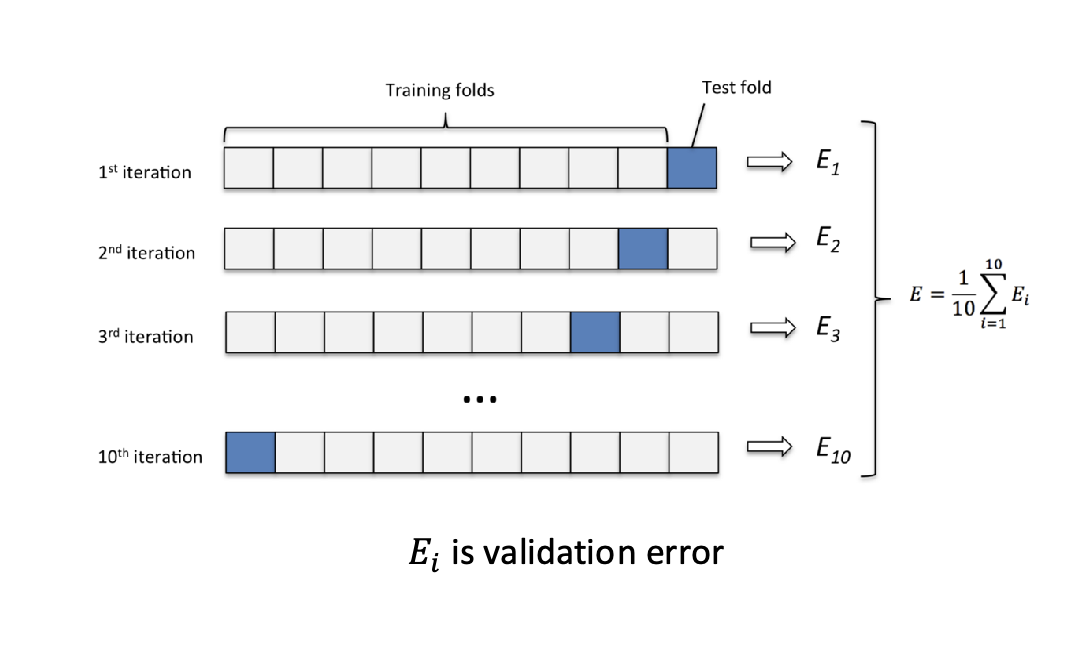
\includegraphics[width=0.55\linewidth]{img/lecture10/crossvalidation.png}
    \caption{K-fold cross-validation procedure.}
\end{figure}



\subsection{Learning Curves}

Learning curves are a fundamental diagnostic tool for understanding how a model improves with more data. When we evaluate a model’s performance, we typically examine two key quantities: the training error and the validation error. As we increase the size of the training set, these quantities can behave differently, providing valuable insights into the model’s learning process and its ability to generalize.

\begin{enumerate}
    \item \textbf{Training Error}: The training error indicates how well the model fits the training data. As the size of the training set increases, the training error usually decreases initially and then stabilizes.

    \item \textbf{Validation Error}: The validation error reflects the model's performance on a separate validation dataset. This quantity helps assess how well the model can generalize to unseen data. Initially, as the training set size increases, the validation error may decrease, indicating that the model is learning relevant structure.
\end{enumerate}


Learning curves are a powerful diagnostic tool. By comparing training and validation 
errors as the dataset size increases, we can determine whether a model is suffering 
from underfitting (high bias) or overfitting (high variance).



\paragraph{How Learning Curves Are Generated}

To generate learning curves, we repeatedly train the model using increasing
amounts of training data and evaluate on a fixed validation set:

\begin{enumerate}
    \item Reserve a validation set of size $v$ from the dataset of size $n$.
    \item For $k = 1, 2, \dots, n-v$:
    \begin{itemize}
        \item Train the model using the first $k$ training samples.
        \item Evaluate training and validation error.
    \end{itemize}
\end{enumerate}


\begin{figure}[H]
    \centering
    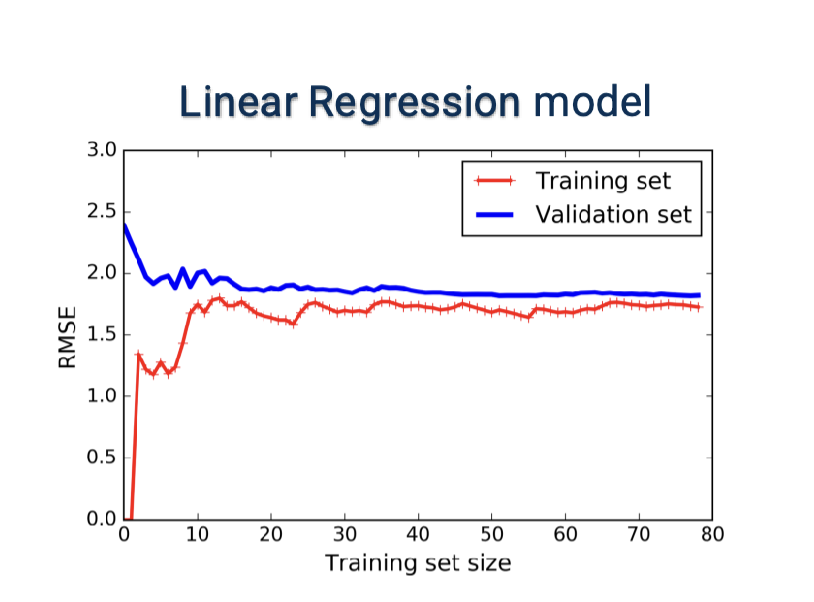
\includegraphics[width=0.5\linewidth]{img/lecture9/Screenshot 2024-09-22 at 6.09.00 PM.png}
     \caption{Underfit linear regression model}
\end{figure}


\begin{figure}[H]
    \centering
    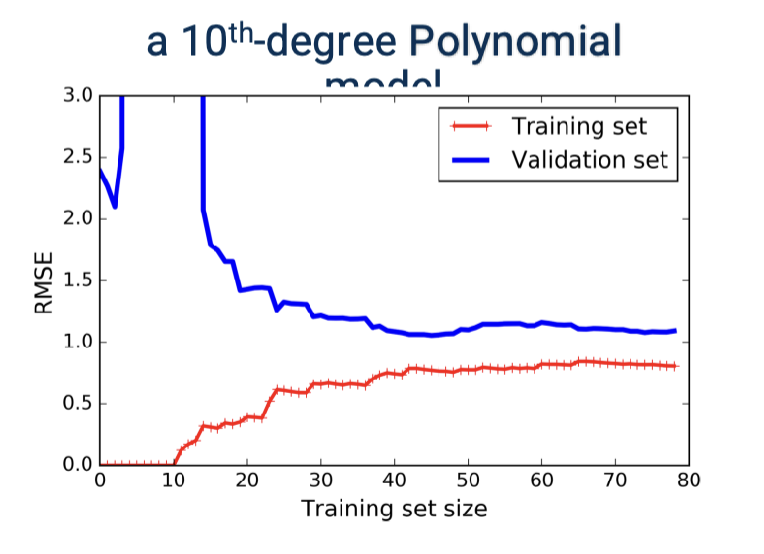
\includegraphics[width=0.5\linewidth]{img/lecture9/Screenshot 2024-09-22 at 6.09.19 PM.png}
     \caption{Overfit polynomial regression model}

    
\end{figure}


From these learning curves, the linear model exhibits consistently high training and validation error, indicating underfitting. The polynomial model achieves lower training error but shows a larger gap between training and validation error, indicating overfitting.


\subsection{Cross-Validation (Interpretation)}

Cross-validation provides a more reliable estimate of generalization performance than a single train/validation split by averaging results across multiple data partitions. This reduces variance in performance estimates and helps prevent overfitting to a specific validation set.



\subsection{Model Complexity vs Prediction Error}


Model complexity in machine learning, often measured by degrees of freedom, refers to a model's capacity to fit data, as seen in polynomial regression. As model complexity increases, training error typically decreases because the model can better fit the training data, potentially reaching a point where training error approaches zero, indicating it captures even the noise. Initially, testing error may also decrease as the model learns relevant patterns, but after a certain complexity level, testing error begins to rise due to overfitting—where the model learns noise instead of generalizable patterns. This highlights the bias-variance tradeoff: low-complexity models may have high bias, leading to oversimplified patterns, while high-complexity models can suffer from high variance, fitting training data well but failing on unseen data. Cross-validation helps identify the optimal level of complexity that minimizes 
generalization error, while regularization mitigates overfitting by penalizing 
excessive complexity.





\begin{figure}[H]
    \centering
    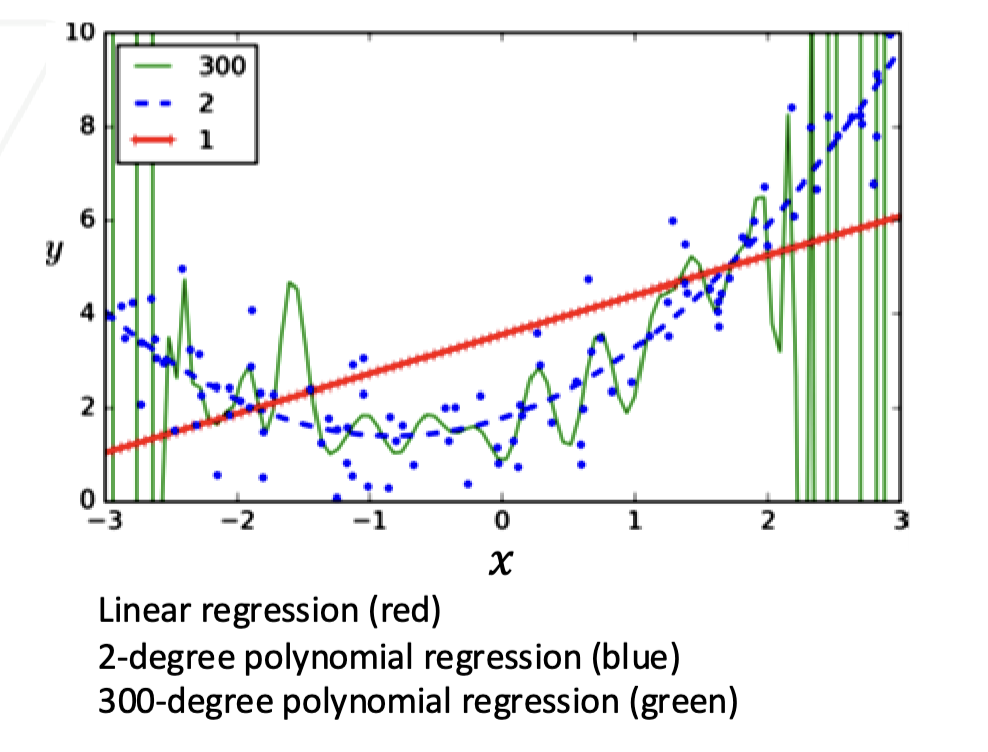
\includegraphics[width=0.5\textwidth]{img/lecture9/Screenshot 2024-09-22 at 6.22.40 PM.png}
    \caption{Diagram depicting the effects of model complexity as degrees of freedom increase}
    
\end{figure}



\begin{figure}[H]
    \centering
    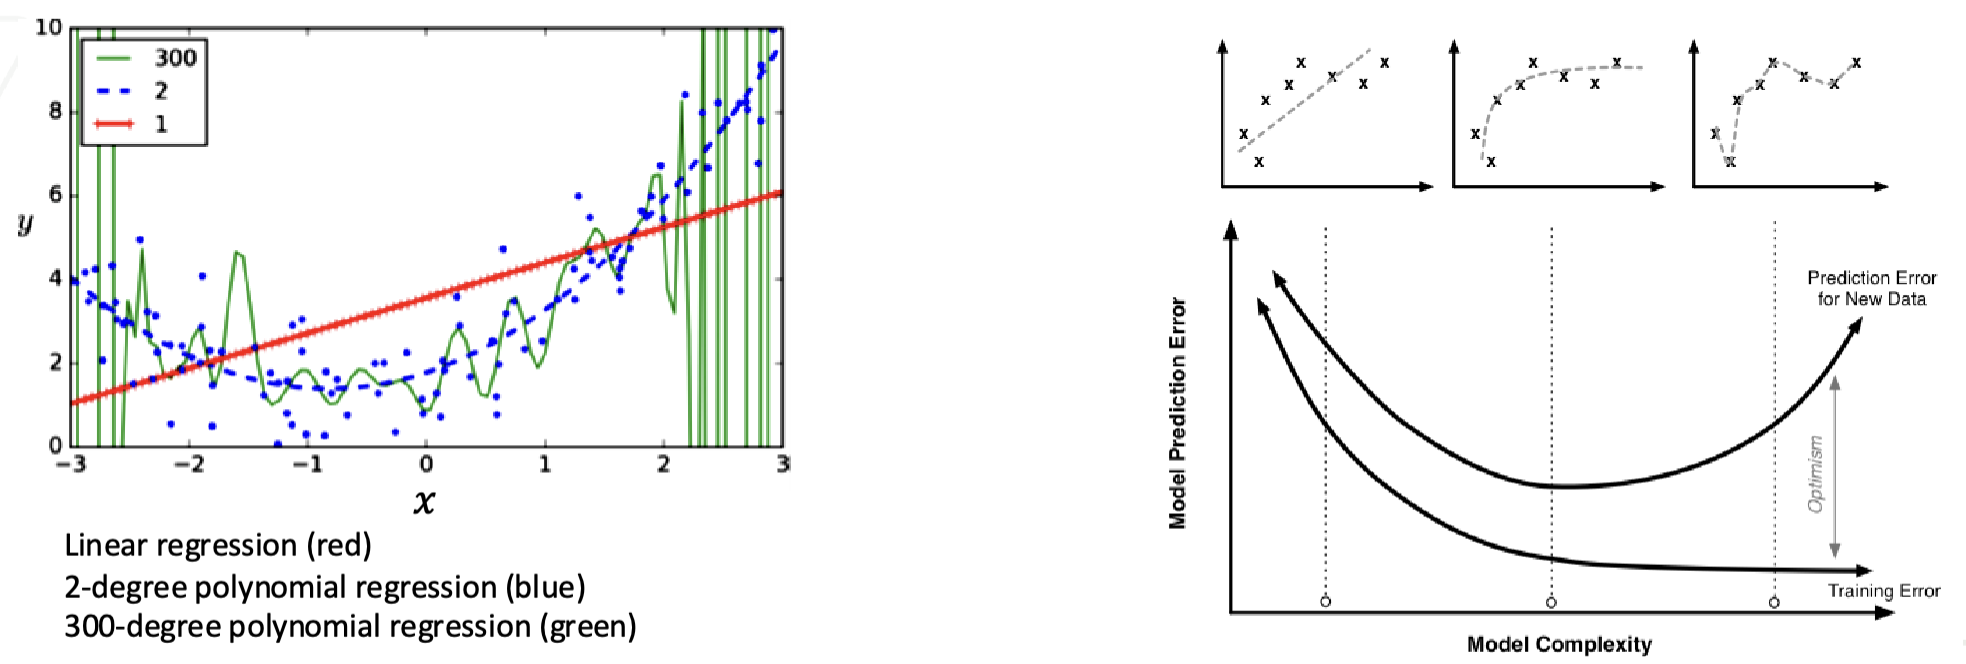
\includegraphics[width=0.55\linewidth]{img/lecture10/modelcomplexity.png}
    \caption{Model complexity vs training and testing error.}
\end{figure}

\section{Model Complexity}

In this final section, we briefly connect the practical ideas from this lecture 
to deeper theoretical concepts from statistical learning theory. The goal is not 
to develop full theory, but to build intuition for why model complexity, data size, 
and regularization are fundamentally linked.

\subsection{Model Complexity}
So far, we have discussed model complexity intuitively using learning curves, 
regularization, and the bias–variance tradeoff. We now take a slightly more 
formal look at what “model complexity” means.

In general, \textit{model complexity} refers to the capacity of a model to fit a wide variety of functions or datasets. As discussed earlier, a more complex model has a higher capacity to capture intricate patterns in the data, but this can also increase the risk of overfitting. One way to think about model complexity is in terms of how many training samples are needed for the model to learn patterns that generalize well to new data, i.e. produce low test error. However, this quantity can be difficult to characterize. Here are a few typical notions:

\begin{itemize}
    \item The degree of the model (e.g., the degree of a polynomial in polynomial regression).
    \item The number of parameters in the model (e.g., weights in a neural network).
    \item The flexibility of the \textit{hypothesis space} the model operates within.
\end{itemize}

The first two are essentially the same in that they describe the \textit{size} of the hypothesis space. In particular, the hypothesis space describes the set of all possible functions the model can select from, given the available data and parameters. For finite spaces, the size is a fair measure of complexity. In fact, in this case we can show that the number of samples needed to adequately fit a model is bounded by the (log of the) size of the space. However, when the space is infinite, as is often the case with continuous models like neural networks, then this notion of counting parameters can break down and we need a more careful measure of complexity.

A classical theoretical way to measure model capacity is the  \textit{VC (Vapnik–Chervonenkis) dimension}. You do not need to compute this in practice, but it provides useful intuition about why complex models require more data. The VC dimension is a theoretical tool used to quantify the capacity of a model by determining the maximum number of points that a model can \textit{shatter}. Shattering means that for a given set of points, the model can perfectly classify all possible binary labelings of those points. The higher the VC dimension, the more complex the model and the larger the class of functions it can represent.

For example, a linear classifier in 2D (like a linear SVM or perceptron) has a VC dimension of 3, meaning it can shatter any set of 3 points in the plane, but not necessarily 4.

%%% Insert a simple illustrative figure showing the shattering concept with VC dimension using the linear classifier example %%%

In practice, models with high VC dimensions are prone to overfitting, as they can represent highly complex decision boundaries. However, models with a VC dimension that is too low may underfit, failing to capture important relationships in the data. The key is to choose a model with an appropriate VC dimension for the problem at hand.

While VC dimension is a powerful theoretical concept, it is not always easy to compute for real-world models. Nonetheless, it serves as a guiding principle: models with higher capacity (e.g., more parameters, higher VC dimension) need more training data to generalize well, and regularization becomes crucial to control overfitting in such cases.

This theoretical perspective reinforces the key message of this lecture: 
as model capacity increases, we must rely on more data, cross-validation, 
and regularization to ensure good generalization.


% \begin{figure}[H]
%     \centering
%     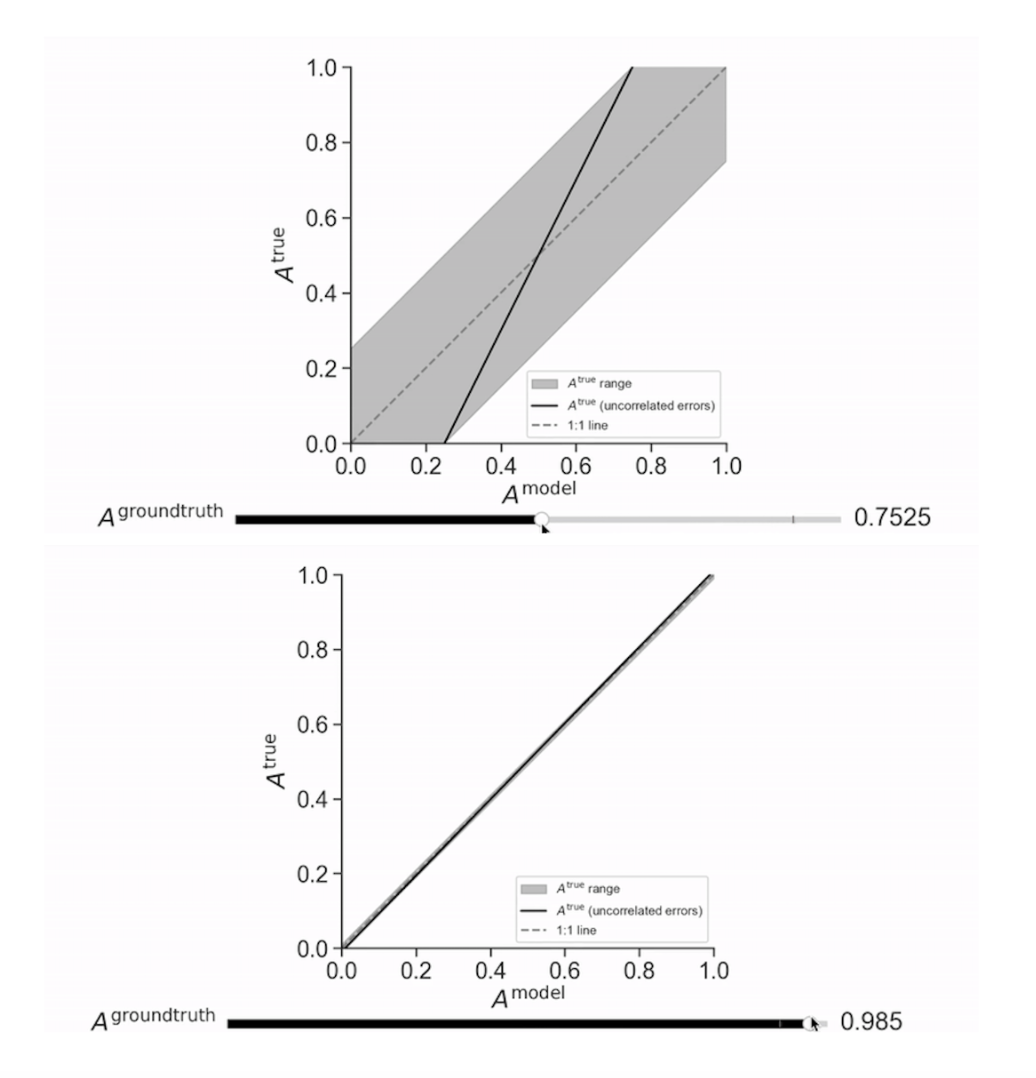
\includegraphics[width=0.85\textwidth]{img/lecture9/P16}
%     \caption{
%     True accuracy vs.\ measured accuracy under label noise.
%     The shaded region shows the range of possible true accuracies that are
%     consistent with a given measured accuracy when ground-truth labels are noisy.
%     As label uncertainty increases, the gap between measured accuracy and true
%     accuracy grows, highlighting why evaluation becomes difficult under ambiguous
%     ground truth.
%     }
%     \label{fig:P16}
% \end{figure}

\subsection{Model Evaluation Under Ambiguous Ground Truth}

So far, we have assumed that every training example has a single correct label. 
However, in many real-world datasets the true label is not perfectly known. 
Different annotators may disagree, labels may be noisy, and some examples may 
naturally belong to multiple categories. This situation is known as 
\textbf{ambiguous ground truth} or \textbf{label noise}.

\subsubsection{Why Accuracy Can Be Misleading}

Standard accuracy assumes that dataset labels are perfectly correct. 
But suppose that a fraction $\epsilon$ of labels are incorrect or uncertain. 
Even a perfect model cannot exceed the accuracy of the noisy labels.

\[
\boxed{
\text{Observed Accuracy} \;\le\; 1 - \epsilon
}
\]

This means a model might appear to plateau at $90\%$ accuracy even if its 
true performance is much higher. In practice, label noise creates uncertainty 
about how measured accuracy relates to the model's true accuracy 
\cite{DBLP:journals/corr/abs-1908-07086, Quesada2025Largescale}.

\begin{figure}[H]
    \centering
    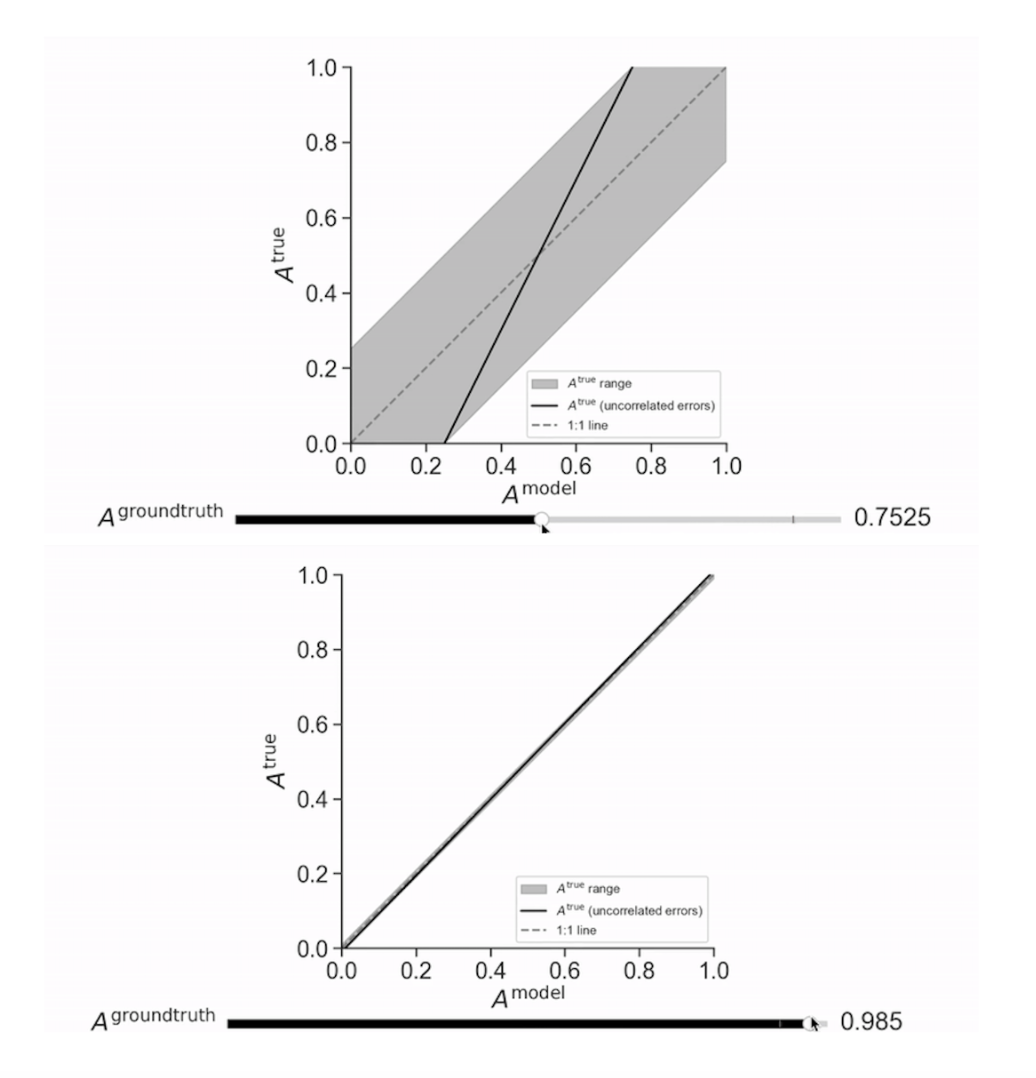
\includegraphics[width=0.75\linewidth]{img/lecture9/P16.png}
    \caption{\textbf{Measured vs.\ true accuracy under label noise.}
    The diagonal line represents perfect labels. When labels contain noise,
    the measured accuracy lies within a band around this line. The shaded
    region shows the range of possible true accuracies for a given measured
    accuracy when ground-truth labels are uncertain.}
    \label{fig:label_noise_accuracy}
\end{figure}

The shaded region illustrates an important takeaway:

\begin{quote}
Measured accuracy is not a single number — it represents a \textit{range of possible true performances}.
\end{quote}

This relationship between measured and true accuracy under noisy labels
has been studied extensively in recent work \cite{DBLP:journals/corr/abs-1908-07086}.


\subsubsection{Human Label Disagreement}

In many tasks, disagreement between humans is not a mistake — it is a 
signal of inherent ambiguity in the data. For example, an image might 
contain features of both a dog and a wolf, or a handwritten digit might 
look like both a 3 and an 8.

Recent research shows that training models using \textbf{distributions 
of human labels} instead of single “hard” labels can improve 
generalization and robustness \cite{cifar10h}.

\begin{figure}[H]
    \centering
    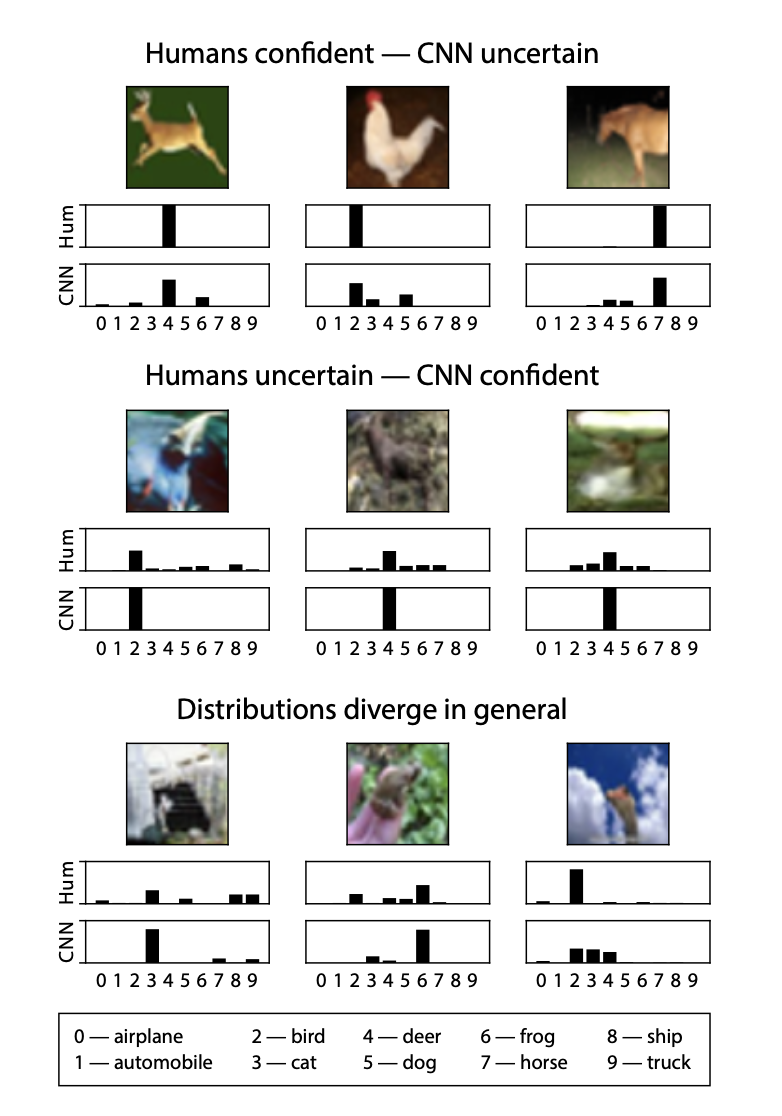
\includegraphics[width=0.85\linewidth]{img/lecture9/P17.png}
    \caption{\textbf{Humans and neural networks disagree in their uncertainty.}
    Top: examples where humans are confident but CNN predictions are uncertain.
    Middle: examples where humans are uncertain but CNN predictions are confident.
    Bottom: examples where both distributions diverge. 
    This highlights that label disagreement contains useful information about
    ambiguity in the data.}
    \label{fig:human_cnn_uncertainty}
\end{figure}

Rather than treating disagreement as noise, we can treat it as 
\textbf{information about uncertainty}.

\subsubsection{Practical Implications}

When labels are noisy or ambiguous, model evaluation becomes more subtle. 
Standard accuracy may \textbf{underestimate true model performance} because the 
model is being judged against imperfect labels. At the same time, models can 
\textbf{overfit to label noise}, memorizing incorrect annotations rather than 
learning generalizable patterns. For this reason, techniques such as 
\textbf{cross-validation} become even more important, and 
\textbf{regularization} plays a key role in preventing models from memorizing 
incorrect labels.

These challenges motivate the use of more robust training and evaluation 
strategies. In practice, modern machine learning often relies on 
\textbf{robust evaluation metrics}, \textbf{label smoothing}, and 
\textbf{probabilistic (soft) labels} that represent uncertainty in annotations 
rather than assuming a single perfectly correct label. These ideas have become increasingly important in modern machine learning,
where large-scale datasets often contain imperfect or ambiguous annotations
\cite{Quesada2025Largescale, cifar10h}. \\ \\
\noindent
\textbf{Key takeaway:} Modern machine learning increasingly treats labels as 
\textit{probabilistic} rather than perfectly correct.

\section{Bias-Variance Tradeoff}

The bias–variance tradeoff provides a theoretical explanation for the 
behavior observed in learning curves and model complexity plots.

Training a Linear Regression model multiple times with different datasets reveals a range of prediction scores, which can provide valuable insights into model performance. The average of these scores, referred to as bias, indicates how consistently the models perform. Models exhibiting high average error are categorized as high-bias, a result of low complexity to capture the underlying patterns in the data. Such models may cause underfitting. In the context of a high-degree Polynomial Regression model, while the bias is significantly reduced due to the model's increased complexity and flexibility, this comes at a cost. The predictions for a given test point can vary dramatically between different polynomial models, indicating a pronounced sensitivity to the training data. This phenomenon, known as variance, arises when the model becomes overly tailored to the nuances of the training dataset, capturing noise rather than the underlying trend. Consequently, high-variance models struggle to generalize effectively to unseen data, resulting in substantially higher prediction errors when applied to new instances. Moreover, this trade-off highlights the delicate balance between bias and variance, underscoring the importance of model selection and regularization techniques to mitigate overfitting/underfitting while still achieving accurate predictions.


\paragraph{Bias–Variance Decomposition}

Let $x$ be a test sample, $f(x)$ the true target, and $\hat{f}(x)$ the model prediction.
The expected squared error can be decomposed as

\[
E[(f(x) - \hat{f}(x))^2]
= \underbrace{(E[\hat{f}(x)] - f(x))^2}_{\text{Bias}^2}
+ \underbrace{E[(\hat{f}(x) - E[\hat{f}(x)])^2]}_{\text{Variance}}
+ \underbrace{\sigma_e^2}_{\text{Irreducible Error}}.
\]

This decomposition explains why increasing model complexity can reduce bias
but increase variance, and motivates the search for an optimal tradeoff.

% \begin{figure}[H]
%     \centering
%     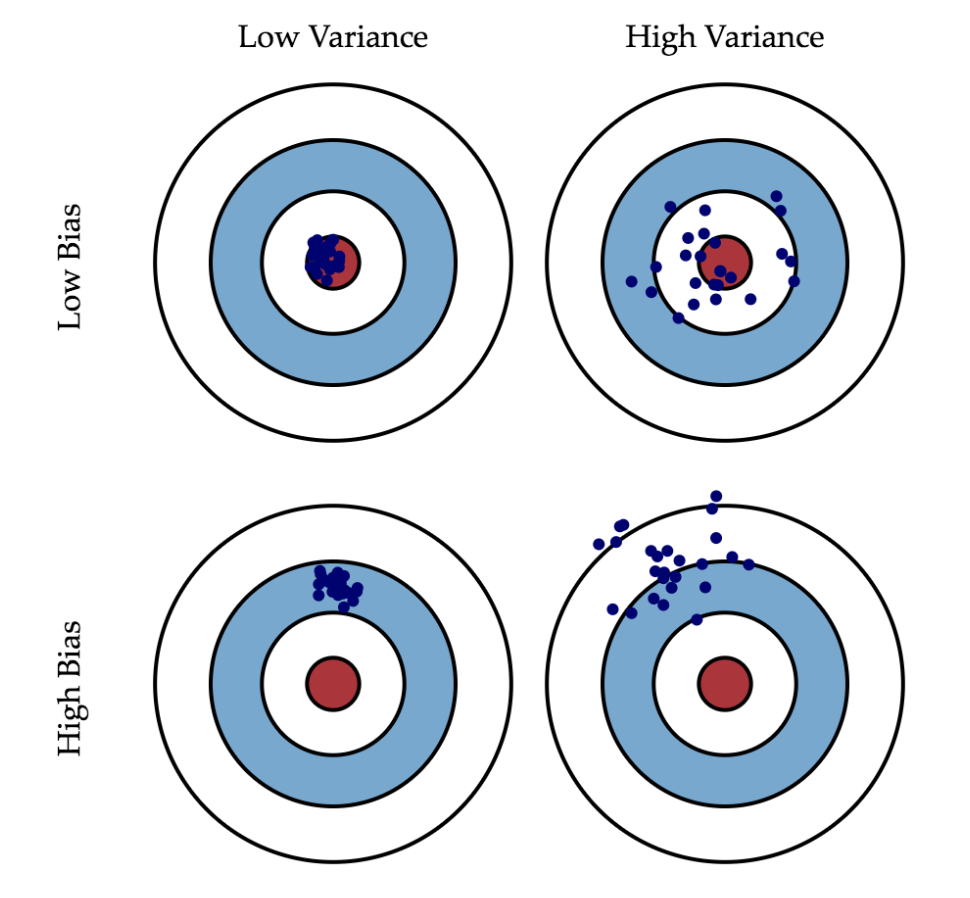
\includegraphics[width=0.45\linewidth]{img/lecture10/biasvariancedarts.png}
%     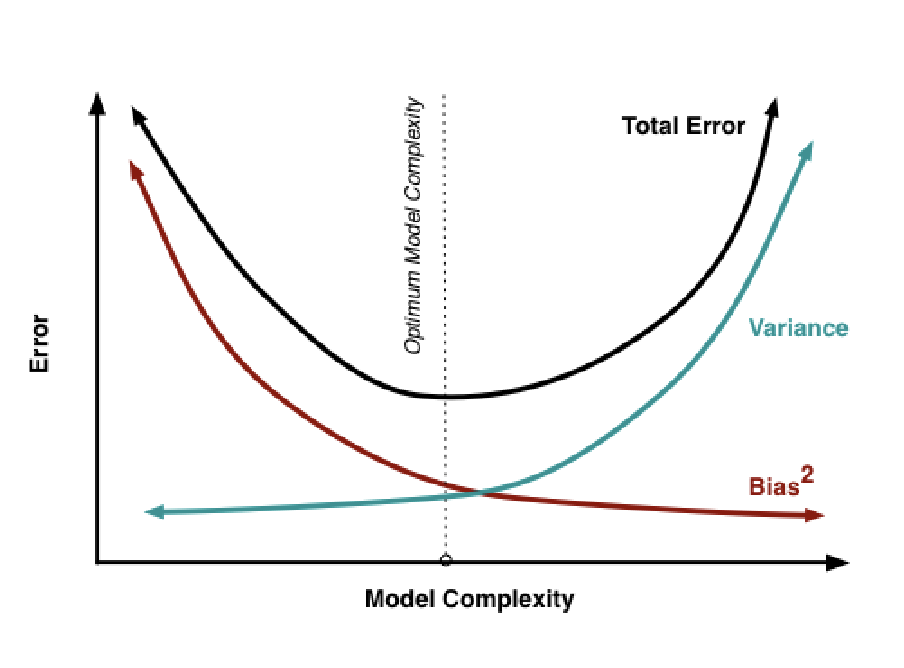
\includegraphics[width=0.45\linewidth]{img/lecture10/biasvariancelc.png}
%     \caption{Bias–variance tradeoff illustrated using dartboard analogy and learning curves.}
% \end{figure}

\begin{figure}[H]
    \centering
    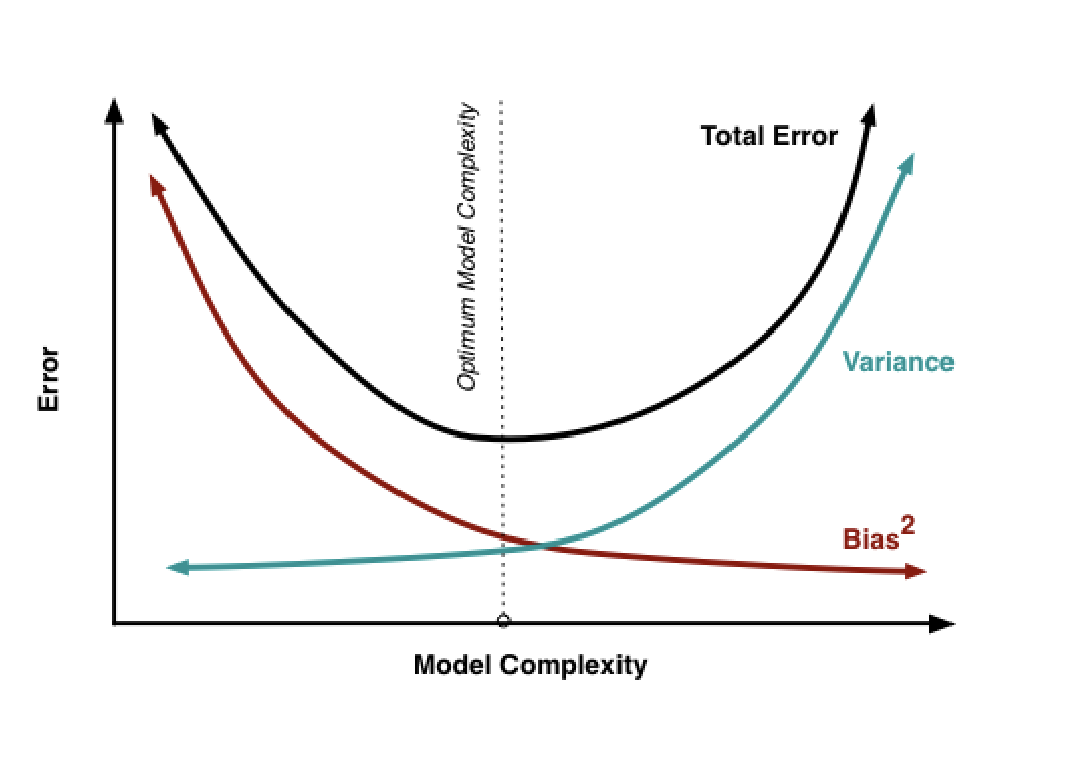
\includegraphics[width=0.5\linewidth]{img/lecture9/Screenshot 2024-09-22 at 6.28.08 PM.png}
    \caption{A diagram depicting the relationship between model complexity and error}
\end{figure}

% A model's error score and its ability to generalize are closely related to its complexity, or flexibility. Finding the optimal complexity involves a tradeoff between Bias and Variance. Bias refers to the error due to overly simplistic assumptions, leading to underfitting, while Variance indicates the error from excessive sensitivity to fluctuations in the training data, resulting in overfitting. Increasing a model's complexity generally decreases Bias, allowing it to capture more intricate patterns in the training data. However, this added complexity can also increase Variance, causing the model to perform well on training data but poorly on unseen data, as it may have memorized the training set rather than learned to generalize. Thus, achieving the right level of model complexity is crucial for optimizing performance, ensuring that the model effectively balances Bias and Variance to generalize well to new data.

\begin{figure}[H]
    \centering
    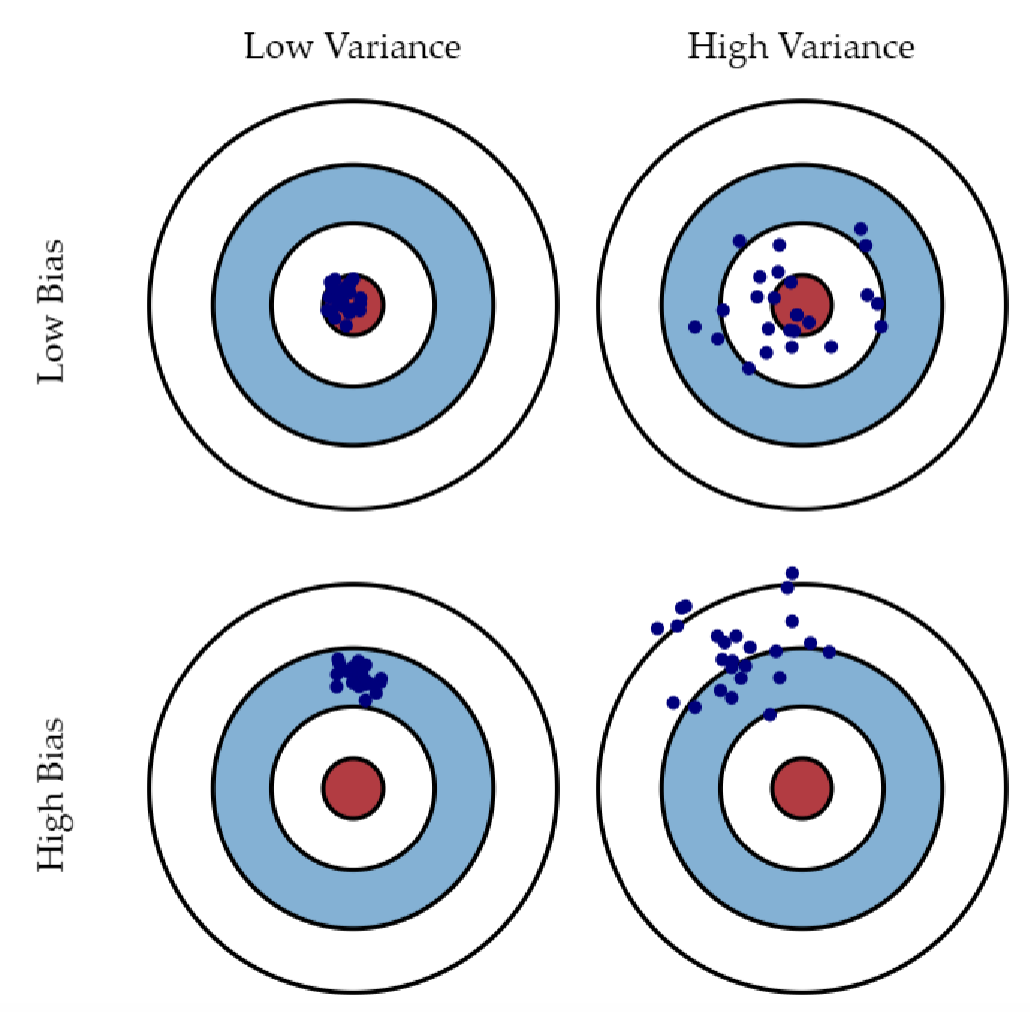
\includegraphics[width=0.5\linewidth]{img/lecture9/Screenshot 2024-09-22 at 6.30.13 PM.png}
    \caption{Diagram depicting the bias-variance tradeoff}
\end{figure}

\begin{figure}[H]
    \centering
    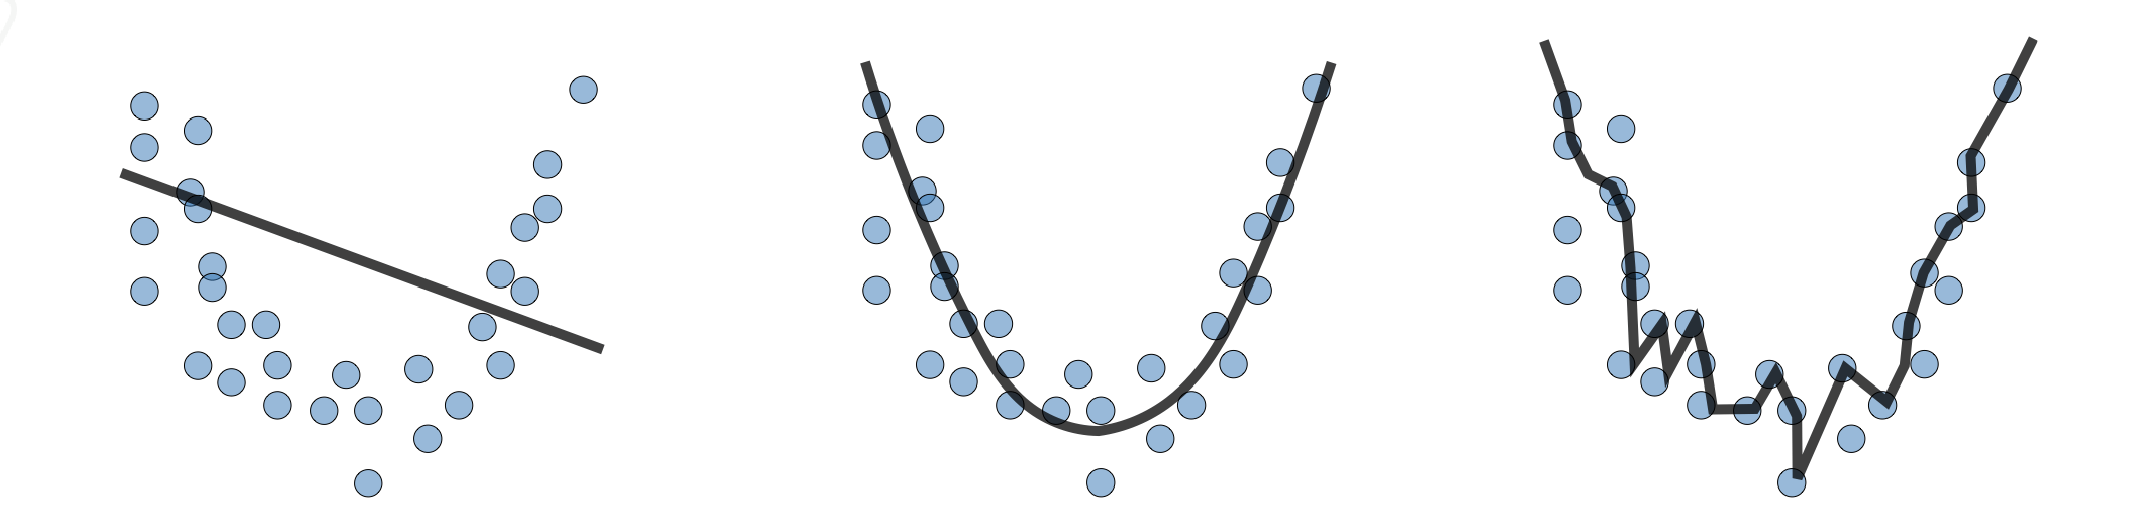
\includegraphics[width=1\linewidth]{img/lecture9/Screenshot 2024-09-22 at 6.41.12 PM.png}
    \caption{Bias--variance decomposition showing how bias decreases and variance increases with model complexity, resulting in a U-shaped total error curve.}
\end{figure}

\begin{table}[H]
    \centering
    \resizebox{\textwidth}{!}{
        \begin{tabular}{lccc}
            & \textbf{Linear Model} & \textbf{Low-Degree Polynomial} & \textbf{High-Degree Polynomial} \\
            \hline
            \textbf{Bias} & Very High & Low & Very Low \\
            \textbf{Variance} & Low & Low & High \\
        \end{tabular}
    }
    \caption{Relationship to the previous figure}
    \label{tab:bias_variance}
\end{table}

This decomposition motivates the bias–variance tradeoff: increasing model complexity typically reduces bias but increases variance.

% We can derive an equation for the error in the model as follows. Assuming $x$ is a test data sample and we have $f(x)$ as the true target, $\hat{f}(x)$ is the models prediction of x, and finally $E[\hat{f}(x)]$ is the average of the target predictions given by the trained model.

% We can formally decompose prediction error into three components. 
% Let $f(x)$ denote the true target, $\hat{f}(x)$ the model prediction, and 
% $E[\hat{f}(x)]$ the expected prediction over many training datasets.
% The expected squared error can be written as:

% \[
% E_{\text{error}}(x) =
% \underbrace{(E[\hat{f}(x)] - f(x))^2}_{\text{Bias}^2}
% +
% \underbrace{E[(\hat{f}(x) - E[\hat{f}(x)])^2]}_{\text{Variance}}
% +
% \underbrace{\sigma_e^2}_{\text{Irreducible Error}}
% \]



\section{Q\&A Section}

\begin{enumerate}

\item \textbf{Question 1:}

When is MAE preferred over MSE?

\begin{enumerate}
    \item When large errors should be heavily penalized
    \item When robustness to outliers is desired
    \item When errors should be squared
    \item When the model must maximize variance explained
\end{enumerate}

\textbf{Answer:} The correct answer is \textbf{B)}.

\textbf{Solution:}

MAE does not square the error, making it less sensitive to large deviations.  
It is preferred when robustness to outliers is important.

\vspace{6pt}

\item \textbf{Question 2:}

Why is RMSE often preferred over MSE for interpretation?

\begin{enumerate}
    \item It penalizes errors more strongly
    \item It has the same units as the target variable
    \item It is always smaller than MSE
    \item It eliminates outliers
\end{enumerate}

\textbf{Answer:} The correct answer is \textbf{B)}.

\textbf{Solution:}

RMSE is the square root of MSE, so it has the same units as the target variable, making it easier to interpret in practice.

\vspace{6pt}

\item \textbf{Question 3:}

What does a negative $R^2$ value indicate?

\begin{enumerate}
    \item Perfect predictions
    \item Better than predicting the mean
    \item Worse than predicting the mean
    \item The model has zero variance
\end{enumerate}

\textbf{Answer:} The correct answer is \textbf{C)}.

\textbf{Solution:}

\[
R^2 = 1 - \frac{SS_{res}}{SS_{tot}}.
\]
If $R^2 < 0$, the model performs worse than predicting the mean of the target variable.

\vspace{6pt}

\item \textbf{Question 4:}

Why are multiple performance metrics often reported together?

\begin{enumerate}
    \item To reduce training time
    \item Because all metrics measure the same thing
    \item Because different metrics capture different aspects of performance
    \item To eliminate overfitting
\end{enumerate}

\textbf{Answer:} The correct answer is \textbf{C)}.

\textbf{Solution:}

Different metrics emphasize different properties, such as sensitivity to outliers or explained variance.  
Using multiple metrics provides a more complete evaluation of model performance.

\vspace{6pt}

\item \textbf{Question 5:}

Which metric is most sensitive to large outliers?

\begin{enumerate}
    \item MAE
    \item MSE
    \item Accuracy
    \item $R^2$
\end{enumerate}

\textbf{Answer:} The correct answer is \textbf{B)}.

\textbf{Solution:}

MSE squares the error:
\[
(\hat{y}_i - y_i)^2,
\]
which heavily penalizes large errors, making it sensitive to outliers.

\vspace{6pt}

\item \textbf{Question 6:}

A model achieves $R^2 = -0.3$ on a test set. What does this mean?

\begin{enumerate}
    \item Perfect predictions
    \item Better than predicting the mean
    \item Worse than predicting the mean
    \item Overfitting has been eliminated
\end{enumerate}

\textbf{Answer:} The correct answer is \textbf{C)}.

\textbf{Solution:}

If $R^2 < 0$, the model performs worse than simply predicting the mean of the data.

\vspace{6pt}

\item \textbf{Question 7:}

Why must the test set never be used during training or hyperparameter tuning?

\begin{enumerate}
    \item It increases computation time
    \item It causes underfitting
    \item It introduces evaluation bias
    \item It reduces training accuracy
\end{enumerate}

\textbf{Answer:} The correct answer is \textbf{C)}.

\textbf{Solution:}

Using the test set during model development leaks information and produces overly optimistic performance estimates.

\vspace{6pt}

\item \textbf{Question 8:}

Suppose $10\%$ of dataset labels are incorrect. What is the maximum achievable measured observed accuracy of a perfect model?

\begin{enumerate}
    \item 100\%
    \item 95\%
    \item 90\%
    \item 80\%
\end{enumerate}

\textbf{Answer:} The correct answer is \textbf{C)}.

\textbf{Solution:}

With label noise $\epsilon$:
\[
\text{Observed Accuracy} \le 1-\epsilon.
\]
If $\epsilon=0.1$, the maximum observed accuracy is $0.9$.

\vspace{6pt}

\item \textbf{Question 9:}

Which method helps estimate generalization performance while using all available data efficiently?

\begin{enumerate}
    \item Cross-validation
    \item Gradient Descent
    \item Newton’s Method
    \item Coordinate Search
\end{enumerate}

\textbf{Answer:} The correct answer is \textbf{A)}.

\textbf{Solution:}

In $k$-fold cross-validation, the model is trained multiple times using different validation splits, and performance is averaged to estimate generalization error.

\vspace{6pt}

\item \textbf{Question 10:}

Consider the model complexity vs.\ prediction error curve below. Which region corresponds to an \textbf{underfitting} model?

\begin{center}
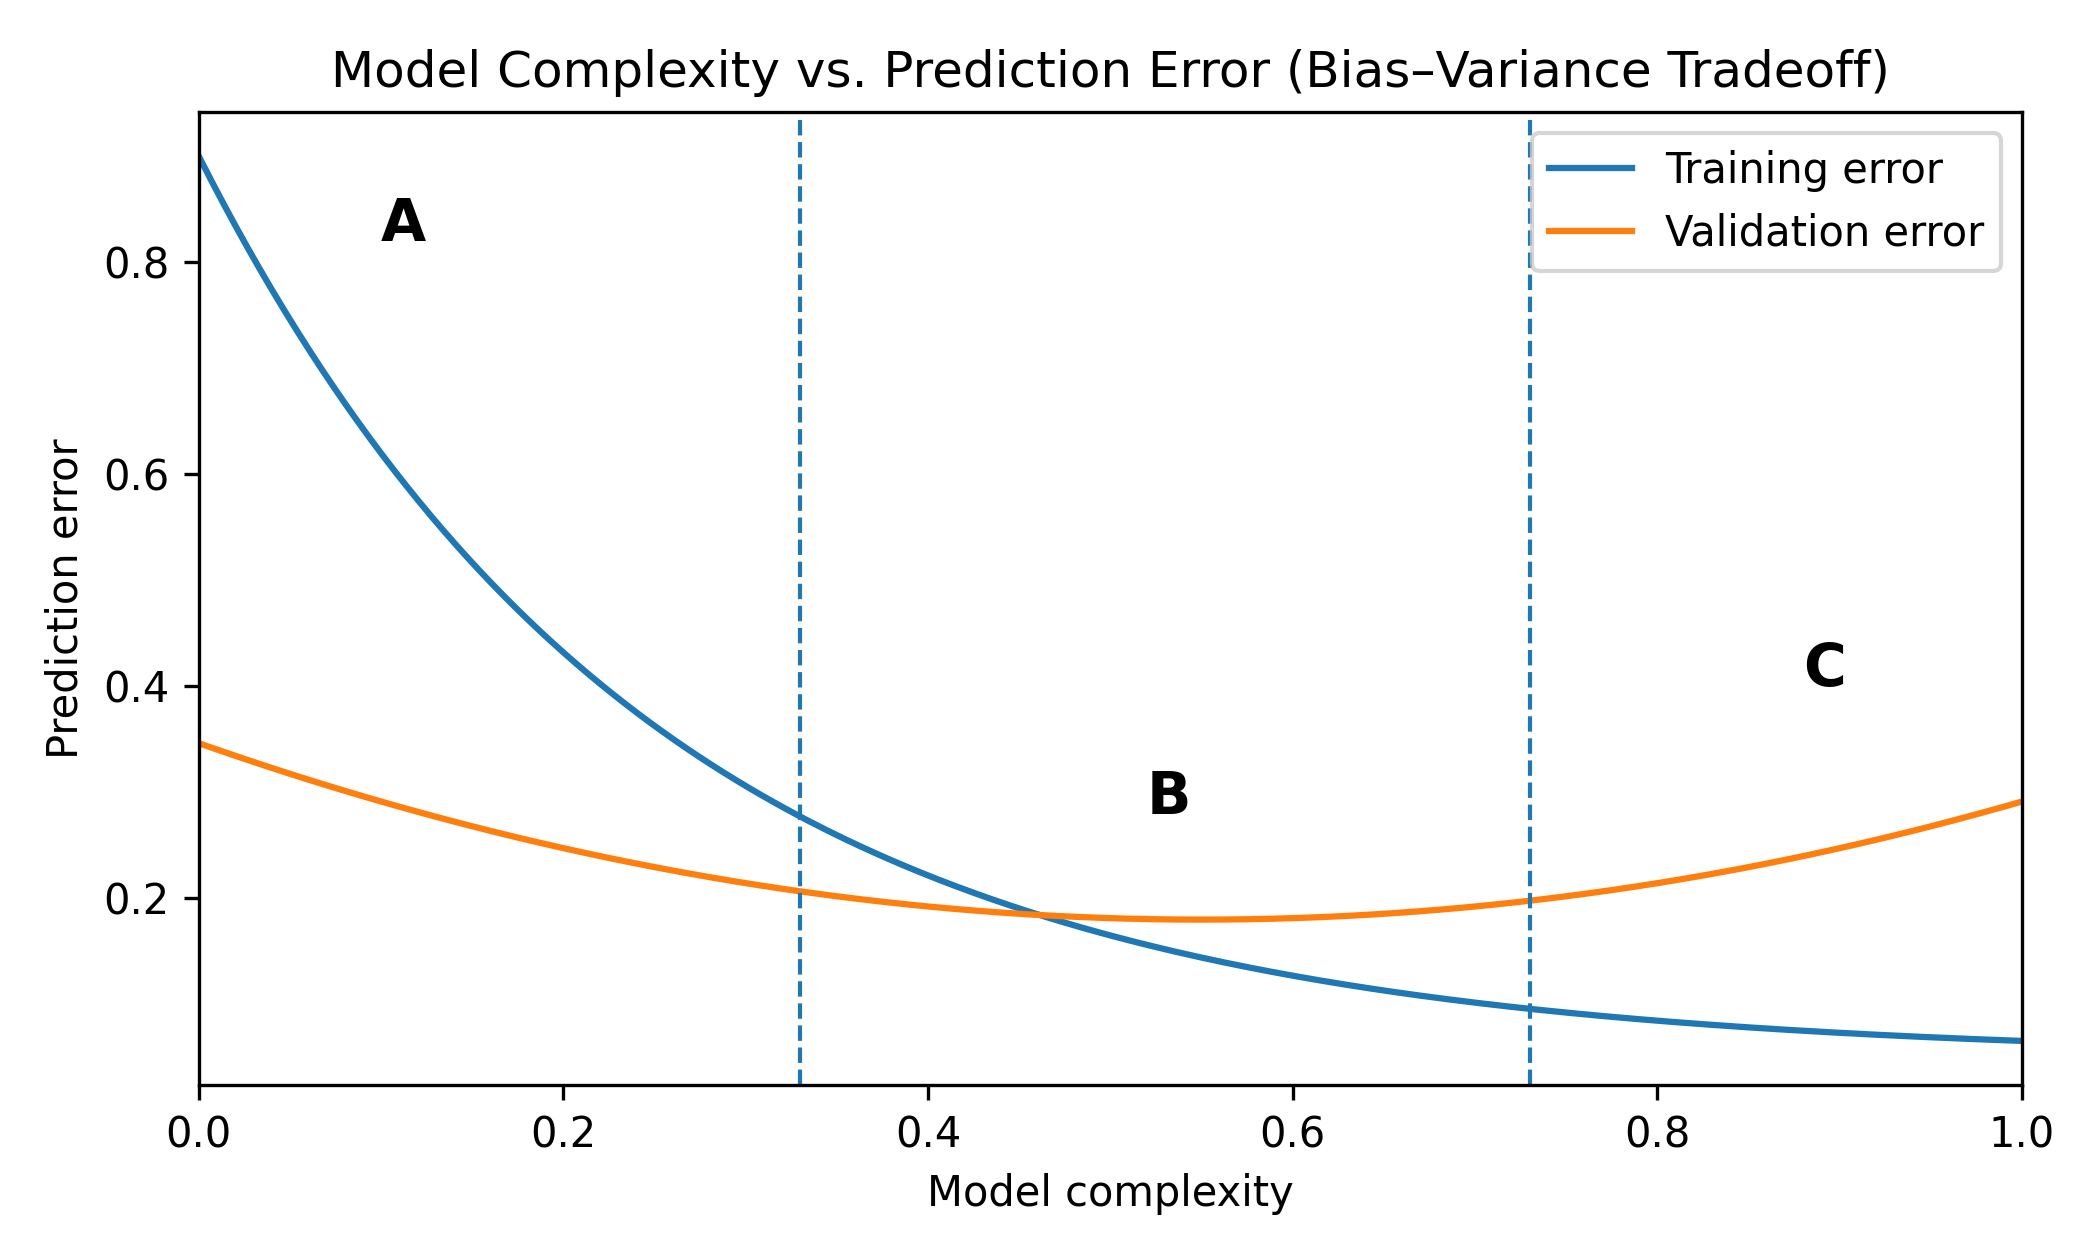
\includegraphics[width=0.6\linewidth]{img/lecture9/qa_bias_variance_curve.png}
\end{center}
This extension to Lecture 9 focuses on evaluating regression models
\begin{enumerate}
    \item Region A (left side)
    \item Region B (middle)
    \item Region C (right side)
    \item All regions equally
\end{enumerate}

\textbf{Answer:} The correct answer is \textbf{A)}.

\textbf{Solution:}

Low-complexity models (left side) have high bias and cannot capture patterns in the data, leading to underfitting.

\item \textbf{Question 11:}

Why should the test set not be used during model development?

\begin{enumerate}
    \item It reduces training time
    \item It prevents bias in performance evaluation
    \item It increases model complexity
    \item It improves convergence
\end{enumerate}

\textbf{Answer:} B)

\textbf{Solution:}

Using the test set during model development leads to overly optimistic performance estimates and poor generalization.

\end{enumerate}

\end{document}
